\documentclass{exam}
\usepackage{graphicx} 


%Format Header and footer
\pagestyle{headandfoot}
\header{\footnotesize Klass:\\Namn:}{\Large\textbf{Prov: Hållbar utveckling: begrepp och reglering}}{\footnotesize HÅLMIJ0\\2024}
\headrule
\footrule
\setlength{\columnsep}{0.25cm}
%\setlength{\columnseprule}{1pt}
\footer{}{Sida \thepage}{}
%\extrafootheight{-2cm}

\begin{document}

\section*{Instruktioner}
Endast ett alternativ är korrekt på flervalsfrågor. Svara kortfattat på övriga frågor.

\subsection*{Poäng}
Varje flervalsfråga ger \textbf{1 poäng}. Övriga frågor anges hur många poäng i frågan.

\section*{Frågor}

\begin{questions}

\question \textbf{Koldioxidekvivalent} är ett ... 
\vspace{2mm}
\begin{checkboxes}
    \choice mått på växthusgaser angett i motsvarande mängd koldioxid
    \choice mått på hur mycket en växthusgas bidrar till global uppvärmning
    \choice mått på koldioxids effekt gällande växthuseffekten
    \choice mått som används för att mäta bilars miljöpåverkan
\end{checkboxes}

\vspace{5mm} 
\hrule 
\vspace{5mm} 

\question Att vi \textbf{exploaterar naturresurser} innebär att ... 
\vspace{2mm}
\begin{checkboxes}
    \choice vi förstör naturen
    \choice vi utnyttjar resurser från naturen
    \choice vi endast använder oss av icke-förnyelsebara resurser
    \choice vi endast använder oss av förnyelsebara resurser
\end{checkboxes}

\vspace{5mm} 
\hrule 
\vspace{5mm} 

\question Att utnyttja resurser från biosfären kallas för /\textbf{ekosystemtjänster}. Dessa delas in i olika kategorier. \textbf{Fotosyntesen} är ett exempel på en ...
\vspace{2mm}
\begin{checkboxes}
    \choice stödjande tjänst
    \choice försörjningstjänst
    \choice reglerande tjänst
    \choice kulturell tjänst
\end{checkboxes}

\vspace{5mm} 
\hrule 
\vspace{5mm} 

\question Att utnyttja resurser från biosfären kallas för /\textbf{ekosystemtjänster}. Dessa delas in i olika kategorier. Att beundra ett vackert landskap är ett exempel på en ... 
\vspace{2mm}
\begin{checkboxes}
    \choice stödjande tjänst
    \choice försörjningstjänst
    \choice reglerande tjänst
    \choice kulturell tjänst
\end{checkboxes}

\vspace{5mm} 
\hrule 
\vspace{5mm} 

\break

\question \textbf{Greenwashing} kan företag eller organisationer anklagas för, det innebär att ...
\vspace{2mm}
\begin{checkboxes}
    \choice att ha ett överdrivet fokus på hållbar utveckling
    \choice att utnyttja statliga subventioner för investeringar i grön teknik
    \choice att använda falsk marknadsföring gällande organisationens arbete för hållbar utveckling
    \choice att använda färgen grönt överdrivet mycket
\end{checkboxes}

\vspace{5mm} 
\hrule 
\vspace{5mm} 

\question I \textbf{avfallstrappan} ...
\vspace{2mm}
\begin{checkboxes}
    \choice Att vi måste prioritera alla steg lika mycket
    \choice Att det översta alternativet är det mest resurssnåla och energieffektiva
    \choice Att vi i samhällskretsloppet främst vill utvinna så mycket energi som möjligt
    \choice Att vi bör jobba nerifrån och upp
\end{checkboxes}

\vspace{5mm} 
\hrule 
\vspace{5mm} 

\question Varför används \textbf{globalhektar} för att mäta \textbf{ekologiska fotavtryck}?
\vspace{2mm}
\begin{checkboxes}
    \choice Det representerar alla länder
    \choice Det är ett hektar med jordens genomsnittliga produktion och visar tydligt hur mycket en person/företag/land förbrukar
    \choice Det mäter hur mycket resurser vi har kvar på jorden
    \choice Det låter bra och viktigt
\end{checkboxes}

\vspace{5mm} 
\hrule 
\vspace{5mm} 

\question Vad menas med virtuellt vatten?
\vspace{2mm}
\begin{checkboxes}
    \choice Allt vatten i Minecraft
    \choice Den vattenförbrukning som inte syns i en färdig produkt gällande dess vattenavtryck
    \choice Det vatten som alltid finns i alla rörsystem och bidrar till vattenavtrycket
    \choice Vatten som inte kan förbrukas och måste tas hänsyn till när vi mäter vattenavtryck
\end{checkboxes}

\vspace{5mm} 
\hrule 
\vspace{5mm} 

\question Vad innebär juridiska styrmedel? (1 poäng)
\vspace{2mm}
\begin{checkboxes}
    \choice Skatter, avgifter och subventioner
    \choice Lagar och regler i ett samhälle
    \choice Straffskalan för olika miljöbrott
    \choice Det som står i Miljöbalken
\end{checkboxes}

\vspace{5mm} 
\hrule 
\vspace{5mm} 

\break

\question Samhällets styrmedel kan delas in i två kategorier: \textbf{juridiska} och \textbf{ekonomiska}. Nämn ett exempel från varje kategori och förklara hur det kan användas för att styra samhället mot en hållbar utveckling. (2 poäng)


\vspace{60mm} 
\hrule 
\vspace{5mm} 

\begin{center}
    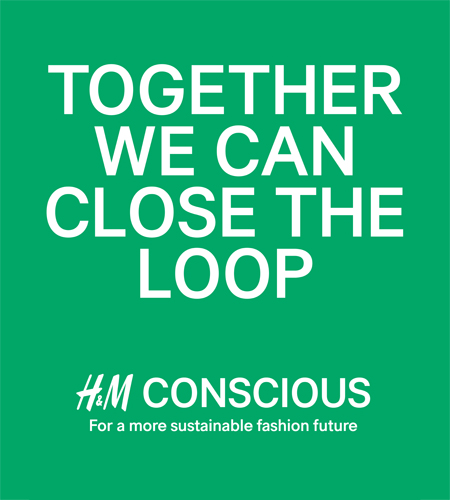
\includegraphics[width=150pt]{image2.png}
\end{center}

\question Bilden är ett exempel på en kampanj som anklagats för att vara \textbf{"greenwashing"}. Vad är problemet med denna typ av reklam? (2 poäng)

\break

\begin{center}
    
\includegraphics[width=400pt]{image.png}
\end{center}

\question Vid exploatering av \textbf{icke-förnyelsebara resurser} används begreppet "peak". Utifrån grafen har vi nått \textbf{"peak-fosfor"}? Vad innebär det och vad medför det för problem? (3 poäng)


\end{questions}

\end{document}

